\documentclass[10pt,conference]{IEEEtran}

\usepackage[utf8]{inputenc}
\usepackage[T1]{fontenc}
\usepackage[english]{babel}
\usepackage{amsmath}
\usepackage{graphicx}
\usepackage{booktabs}
\usepackage{array}
\usepackage{xcolor}
\usepackage{microtype}
\usepackage{titlesec}
\usepackage{fontawesome5}
\usepackage[hidelinks]{hyperref}

\graphicspath{{figures/}{../artifacts/figures/}}
\definecolor{accent}{HTML}{2878B5}
\definecolor{accentdark}{HTML}{174F73}
\definecolor{muted}{HTML}{555555}
\newcommand{\code}[1]{\texttt{\small #1}}
\newcommand{\contactsep}{\hspace{0.4em}{\color{muted}\textbar}\hspace{0.4em}}
\newcommand{\decision}[1]{\textbf{\color{accent}#1}}
\renewcommand{\arraystretch}{0.94}
\setlength{\textfloatsep}{6pt plus 1pt minus 2pt}
\setlength{\floatsep}{5pt plus 1pt minus 2pt}
\setlength{\intextsep}{5pt plus 1pt minus 2pt}
\titleformat{\section}
  {\normalfont\bfseries\color{accentdark}}
  {\thesection.}{0.45em}{}
\titleformat{\subsection}
  {\normalfont\bfseries\color{accent}}
  {\thesubsection}{0.45em}{}
\titlespacing*{\section}{0pt}{1.1ex plus 0.3ex}{0.5ex}
\titlespacing*{\subsection}{0pt}{0.8ex plus 0.2ex}{0.3ex}

\title{\textit{Predicting a Player's Final Ranking}\\
\large from Game Statistics}

\author{
\IEEEauthorblockN{\textbf{Rostand Surel}}
\IEEEauthorblockA{\textit{Data Scientist} --- Paris, France\\[0.3em]
\href{tel:0753356106}{\faPhone\ 075-335-6106}\contactsep
\href{mailto:rostandsurel@yahoo.com}{\faEnvelope\ rostandsurel@yahoo.com}\contactsep
\href{https://linkedin.com/in/rostand-surel}{\faLinkedin\ linkedin.com/in/rostand-surel}\\
\href{https://github.com/Manda404}{\faGithub\ github.com/Manda404}\contactsep
\href{https://Manda404.github.io}{\faGlobe\ Portfolio}\contactsep
\faMapMarker*\ Paris, France}
}

\begin{document}
\maketitle

\begin{abstract}
In this report, I present the complete analysis and prediction pipeline that I
built to estimate a player's team's normalized final ranking from Battle Royale
post-match statistics. I first clarify missing-value codes, incomplete match
structure, and actual feature availability. I then create business-oriented
features, retain 16 variables, and keep every player from the same match in the
same validation group. I compare five model families under identical
conditions. CatBoost achieves the lowest mean absolute error (MAE), 0.06145,
versus 0.26788 for the global-median baseline. Snapping predictions to rankings
that are possible within each match gives 0.06098 out-of-fold MAE. The frozen
model then achieves 0.06080 MAE on the grouped holdout. Finally, I reuse the
saved model, without retraining, to generate the 5,000 submission predictions.
\end{abstract}

\begin{IEEEkeywords}
tabular regression, Battle Royale, exploratory analysis, feature engineering,
grouped validation, CatBoost, data leakage
\end{IEEEkeywords}

\section{Problem and data}

\textbf{I start from the business problem.} Around one hundred players take
part in a match, but each row describes only one player after the match.
\code{gameId} identifies the match and \code{teamId} its team; solo, duo,
squad, and special modes change action context and group size. The target
\code{winRankPercentage} is 1 for first place and 0 for last place. It depends
on \code{maxRank}, not on \code{numTeams}.

The 30 train columns cover combat, mobility, resources and survival, match
context, external rankings, identifiers, and the target. Train contains 50,000
rows, 30,983 \code{gameId}s, and 16 modes; unlabeled test contains 5,000 rows,
4,431 matches, and 10 modes. The brief assigns train to January--April 2024
and test to May 2024.

\begin{table}[!h]
\centering
\caption{Properties of the supplied data.}
\label{tab:data}
\small
\begin{tabular}{@{}lrr@{}}
\toprule
 & \textbf{Train} & \textbf{Test}\\
\midrule
Player rows & 50,000 & 5,000\\
Columns & 30 & 29\\
Numeric columns & 25 & 24\\
Categorical/text columns & 5 & 5\\
Raw missing values & 0 & 0\\
Exact duplicates & 0 & 0\\
Distinct matches & 30,983 & 4,431\\
Distinct modes & 16 & 10\\
\bottomrule
\end{tabular}
\end{table}

\subsection{Quality, sampling, and outliers}

\textbf{Clean does not mean reliable.} Although Table~\ref{tab:data} contains
neither raw missing cells nor exact duplicates, it includes business
conventions: \code{rankPts=-1} affects 38.38\% of rows, and conditionally zero
ranking values affect 59.68\%. I convert these sentinels to missing values with
availability flags and exclude external rankings from the model. I group the 93
malformed \code{gameId}s conservatively so that the same match cannot cross
partitions. I document rare gameplay inconsistencies rather than correcting
them arbitrarily.

Figure~\ref{fig:data-audit} gives scale to these decisions. Train observes only
1.61 players per match on average, at most eight, and only 2.34\% of rows have
an observed teammate. In addition, the median date span within one
\code{gameId} is 45.03 days. I therefore cannot faithfully reconstruct a team
or chronology from the observed sample.

\begin{figure}[!t]
\centering
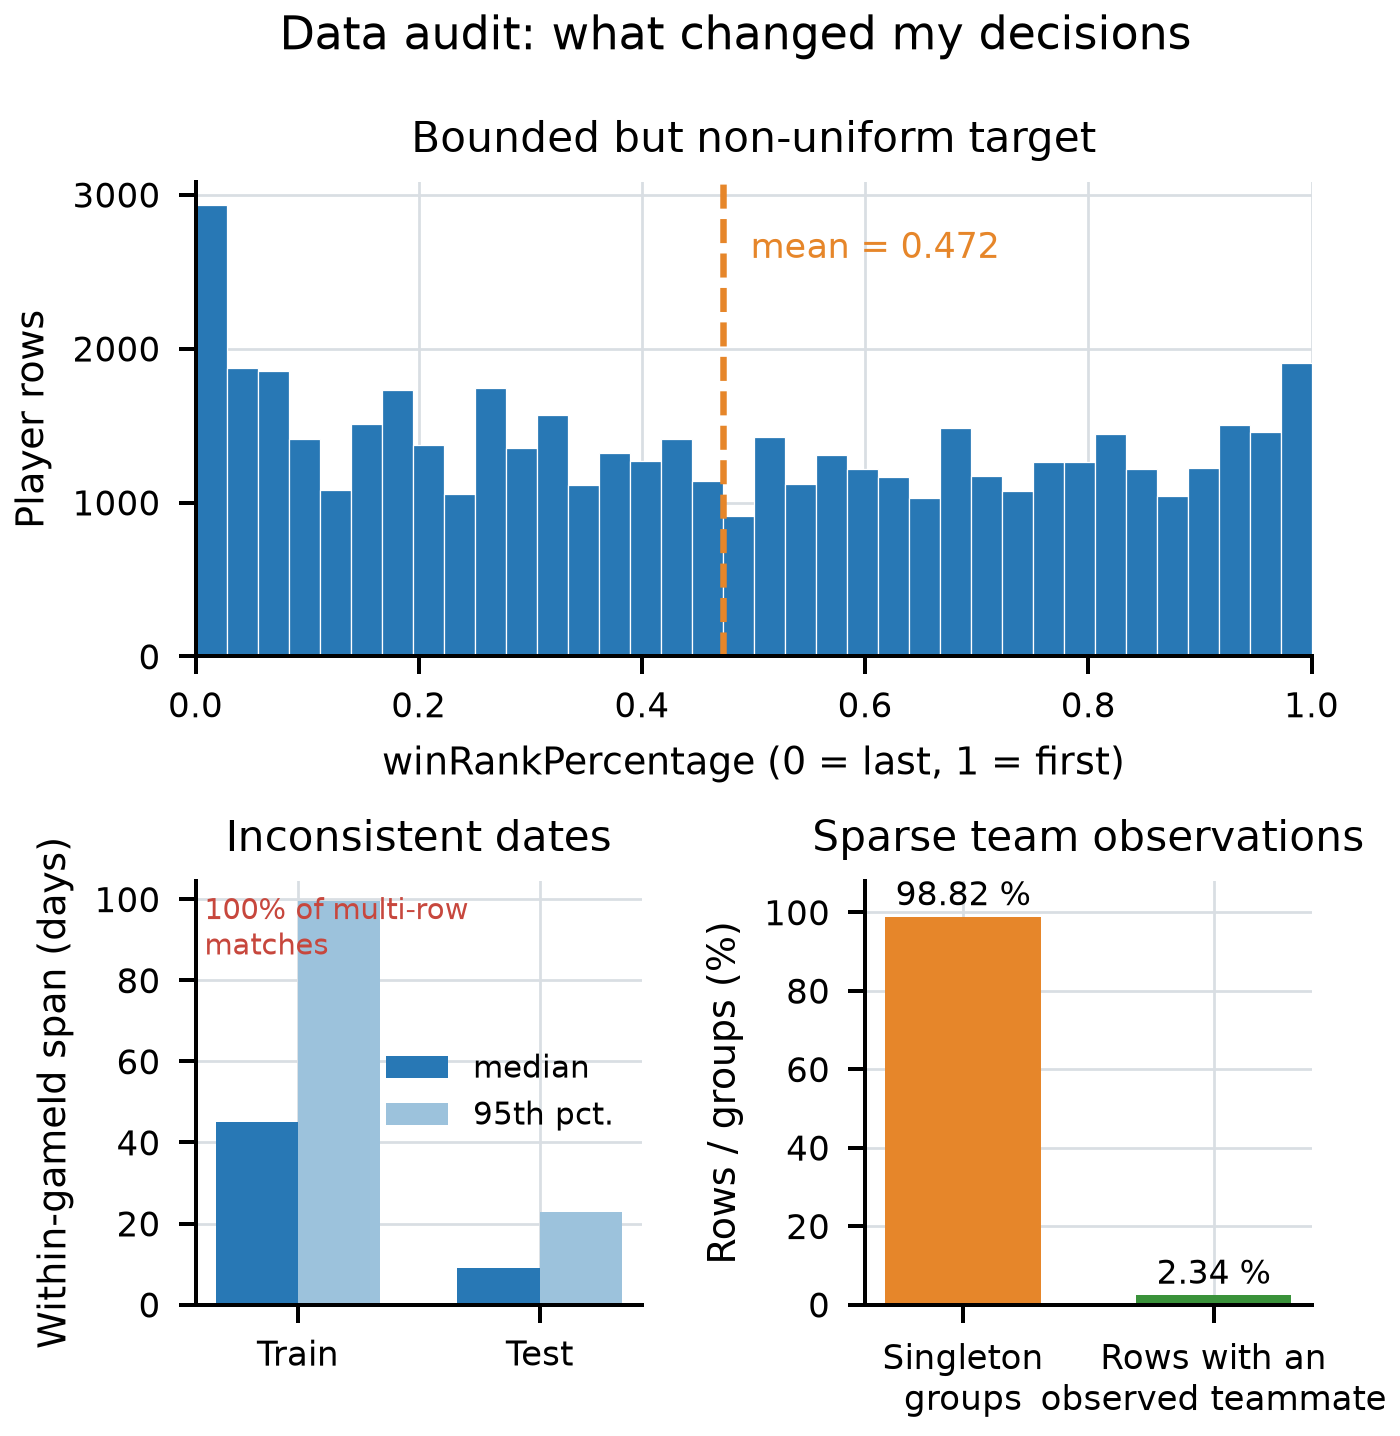
\includegraphics[width=0.92\columnwidth]{01_data_audit.png}
\caption{The target spans $[0,1]$, but date assignment and team coverage
contradict two natural assumptions. I use these findings to determine features
and validation.}
\label{fig:data-audit}
\end{figure}

\textbf{A statistical outlier is not automatically an error.} The standard
$1.5\times IQR$ rule flags 24.91\% of \code{rideDist} and 11.59\% of
\code{kills}. Both variables are concentrated at zero, so their global lower
quartile is zero and the threshold becomes artificially low. When I calculate
IQR only on positive values, those rates fall to 0.66\% and 1.20\%. I retain
rare maxima because removal or winsorization would erase performance signal. I
still flag the 53 rows with \code{kills>0} and \code{damages=0}, and the 102
rows with combat activity but zero distance, as business anomalies.

\subsection{Exploration and drift}

\textbf{The dominant signal is behavioural.} The target mean is 0.4723, its
median is 0.4579, and its standard deviation is 0.3074. Walking distance is
the clearest behavioural signal: its Spearman correlation with the target is
0.866, and mean ranking rises from 0.093 to 0.870 from the first to the last
walking-distance decile (Figure~\ref{fig:profiles}). I interpret this as a
marker of progression and survival, not as a causal effect of walking.

Combat is also informative but less discriminative: damages and kills have
correlations of 0.449 and 0.425. Resources tell a complementary story.
\code{killRank} has a strong $-0.715$ target association, but it is computed
after the match. I therefore distinguish a behavioural contract without it
from an enriched post-match contract.

\begin{figure}[!t]
\centering
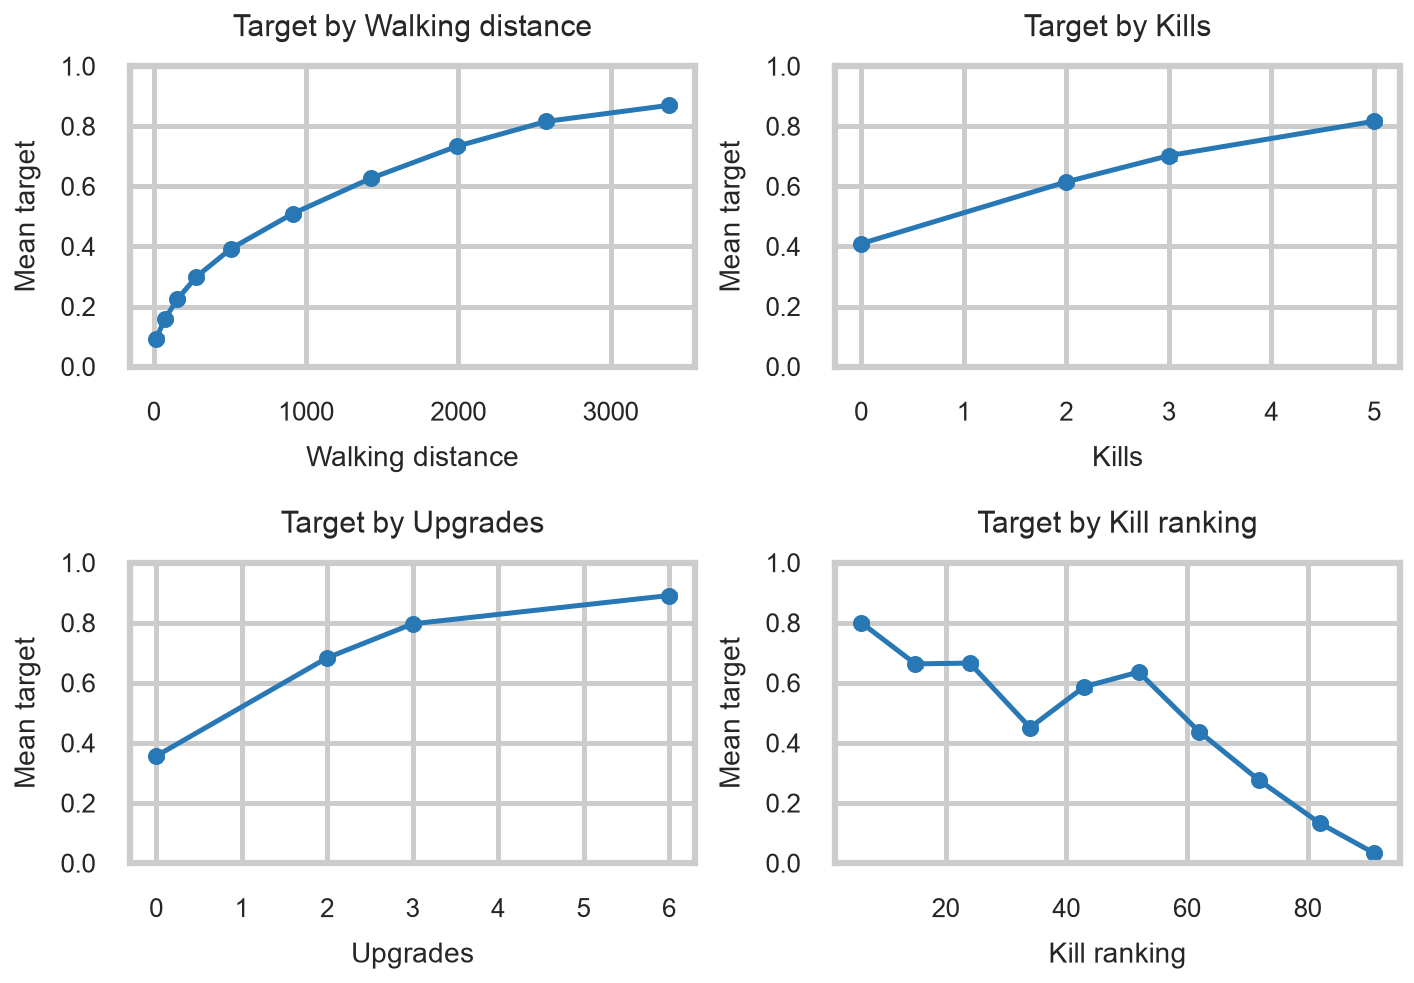
\includegraphics[width=0.94\columnwidth]{06_eda_profiles.png}
\caption{Mean ranking by quantile. Mobility, kills, and upgrades increase with
performance, whereas \code{killRank} decreases sharply. These nonlinear shapes
motivate tree-based models.}
\label{fig:profiles}
\end{figure}

I also compare train and test without using a test target. Maximum numeric and
categorical PSI are 0.00509 and 0.00844, while adversarial validation reaches
ROC AUC 0.4933. Figure~\ref{fig:drift} therefore shows no material shift for
the measured feature contract. It does not prove future performance stability,
and inconsistent dates cannot support a temporal interpretation.

\begin{figure}[!t]
\centering
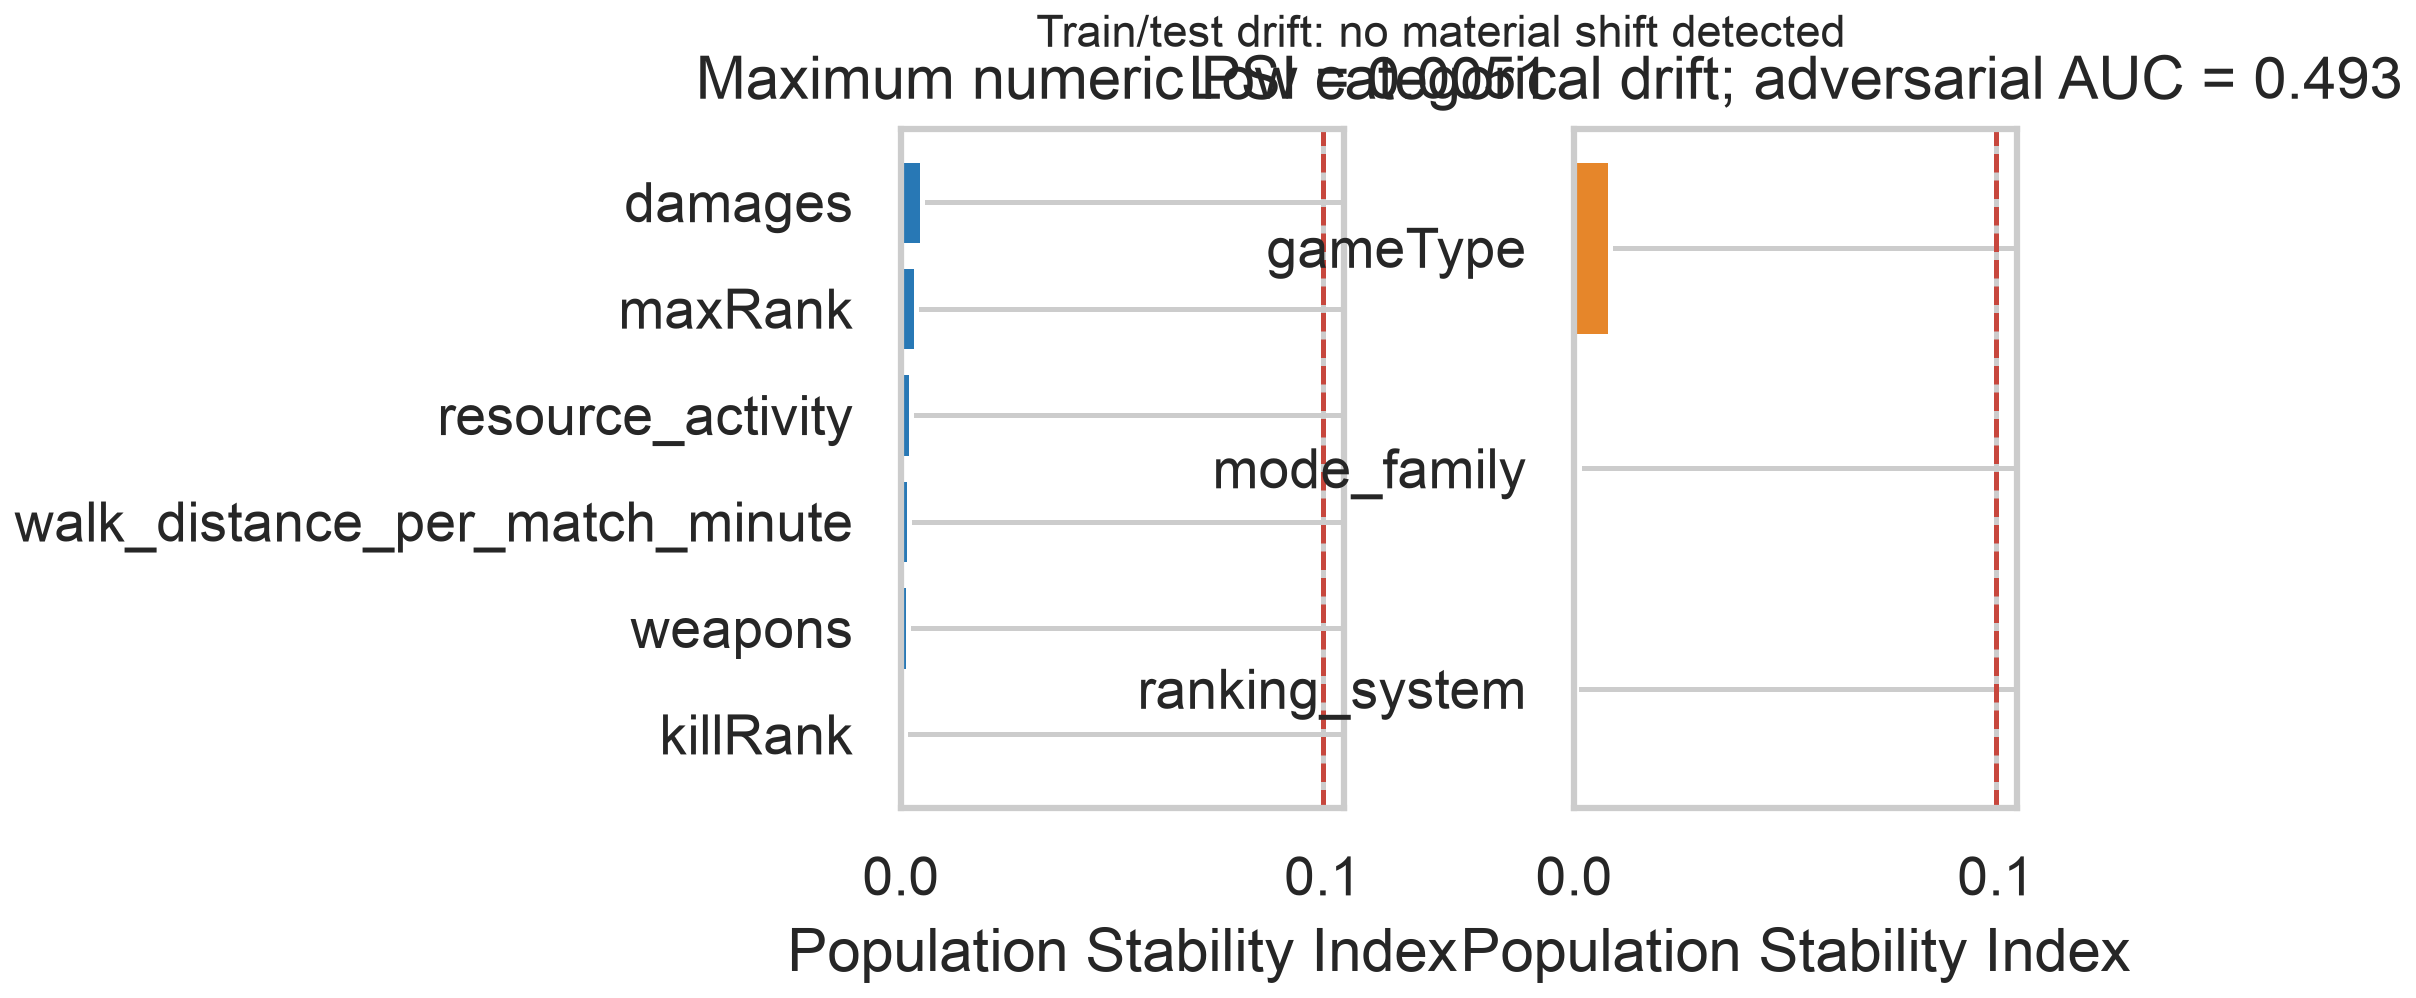
\includegraphics[width=0.90\columnwidth]{05_drift_diagnostics.png}
\caption{PSI values stay well below the 0.1 diagnostic guide, and the
adversarial classifier cannot separate train from test. This supports feature
comparability, not a claim about future performance.}
\label{fig:drift}
\end{figure}

\section{Method}

\subsection{Validation before modeling}

\textbf{I define validation before comparing models.} A row-random split treats
players as independent, yet 56.64\% of its validation rows come from already
seen matches. I keep each match on one side of a partition. First, I freeze a
9,872-row grouped holdout; the remaining 40,128 rows alone feed 5-fold
\code{GroupKFold}, so no \code{gameId} crosses a partition.

The purged pseudo-temporal split removes leakage but drops 8,536 rows and does
not repair contradictory dates. I retain it only as a stress test; grouped
validation is the primary evidence. A sensitivity study over 3, 5, 7, and 10
folds confirms CatBoost in all 25 partitions. I retain five folds: about 8,026
rows per fold, while seven folds cost 52\% more for only 0.000189 nominal MAE
improvement.

\begin{figure}[!t]
\centering
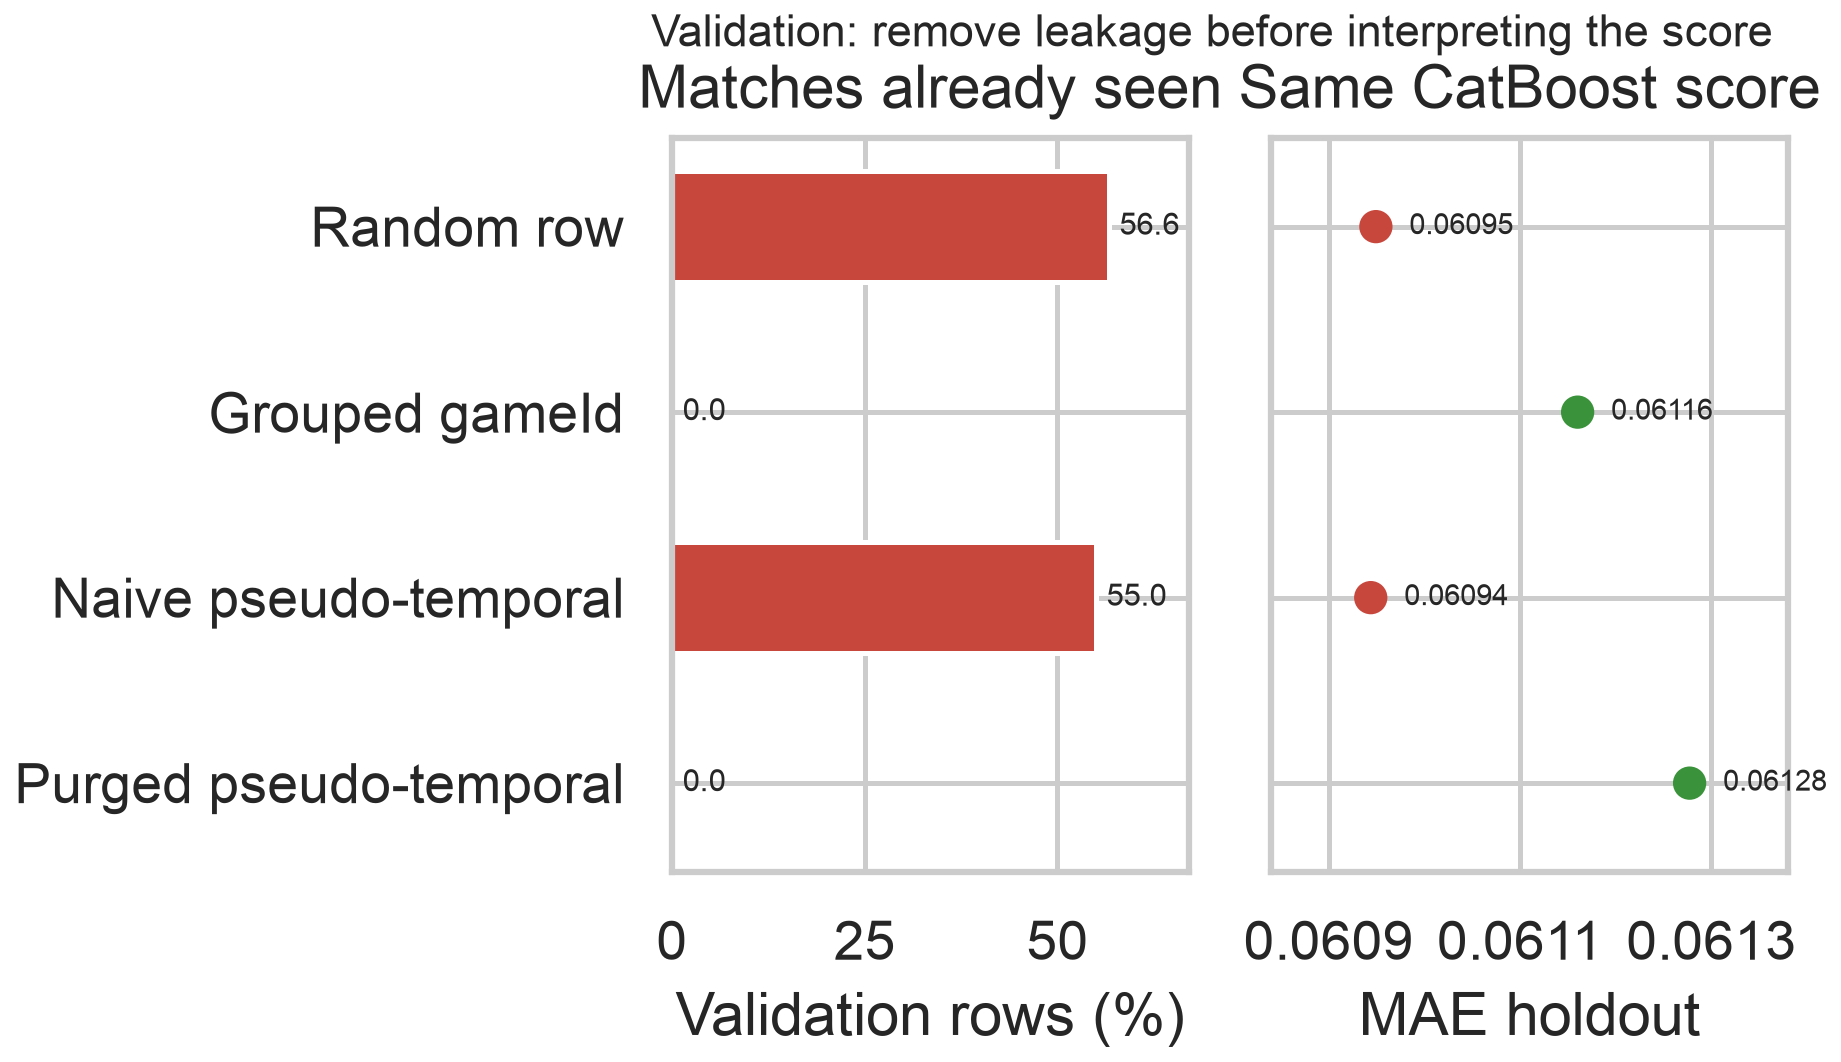
\includegraphics[width=0.90\columnwidth]{03_validation_protocol.png}
\caption{A similar score does not make a split valid. Grouping and purging
remove seen matches; my primary protocol prioritizes valid estimation.}
\label{fig:validation}
\end{figure}

\subsection{Features and model selection}

\textbf{I keep the contract deliberately compact.} I retain eight raw measures
and create four summaries: \code{walkDist}/(\code{gameTime}/60), damage per
kill (zero with no kill), combat activity $=$ kills $+$ assists $+$ knocks, and
resource activity $=$ weapons $+$ upgrades $+$ heals. Three indicators encode
solo, duo, and squad, with special modes as reference. \code{killRank} is the
sixteenth feature in the enriched contract.

The ablation in Figure~\ref{fig:ablation} confirms that mobility provides the
main behavioural gain, while combat and resources add stable signal. Without
\code{killRank}, MAE is 0.09266; with it, MAE is 0.06150. Both scenarios are
post-match, but the latter uses particularly strong final-match information.

\begin{figure}[!t]
\centering
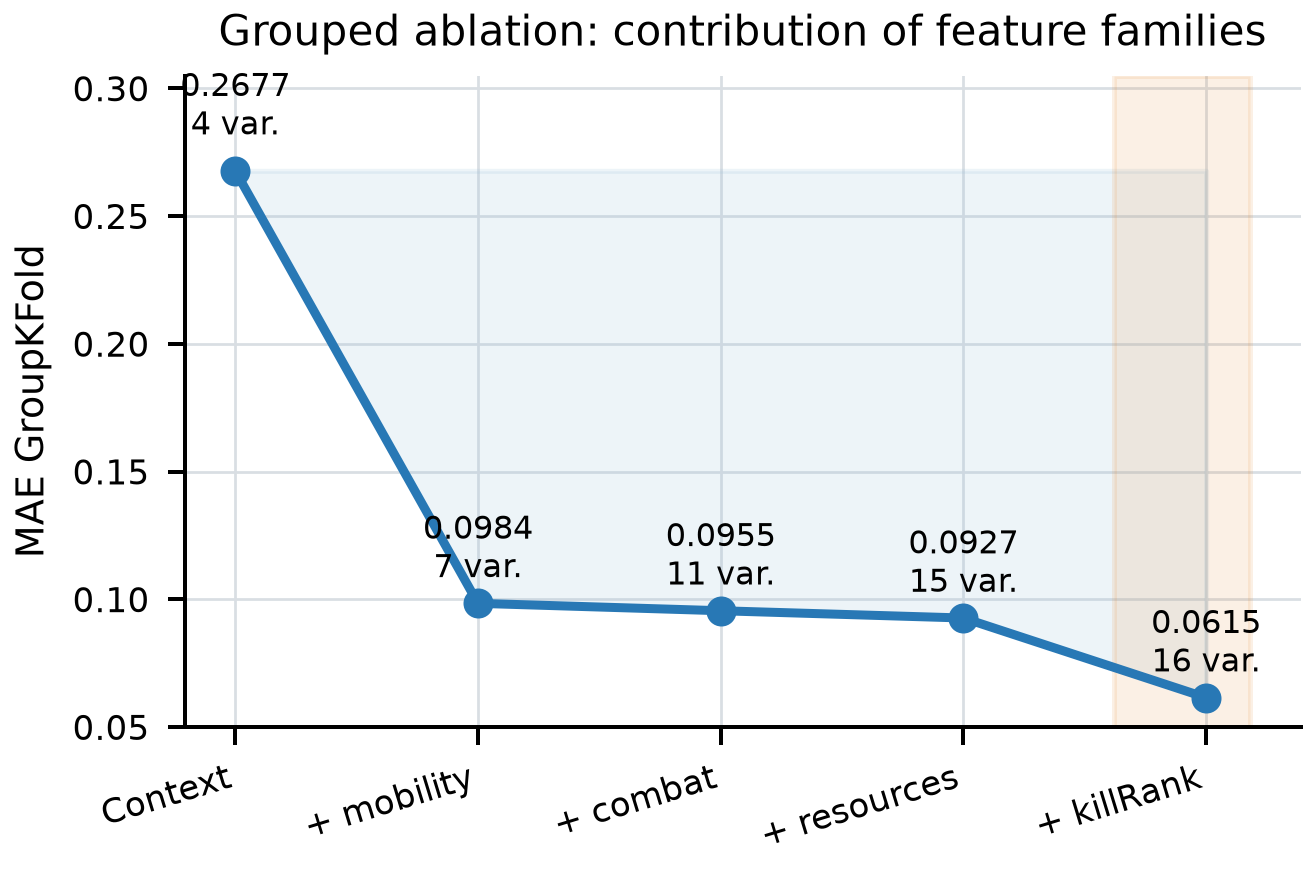
\includegraphics[width=0.90\columnwidth]{02_feature_ablation.png}
\caption{Progressive grouped-validation ablation. I retain each family for its
reproducible gain; the final step quantifies the central role of post-match
\code{killRank}.}
\label{fig:ablation}
\end{figure}

I compare mean/median Dummy regressors, Ridge, Random Forest, XGBoost,
LightGBM, and CatBoost on the same 16 features, rows, and folds. The primary
criterion is
\[
\operatorname{MAE}=\frac{1}{n}\sum_{i=1}^{n}\left|y_i-\hat y_i\right|.
\]
MAE measures the average ranking gap on the natural $[0,1]$ scale, giving each
player equal weight. Unlike RMSE, it is not dominated by a few extreme errors;
I nevertheless inspect those errors separately. Fold stability, the
train--validation gap, RMSE, and $R^2$ complete the decision.

\section{Results, interpretation, and limitations}

\begin{table}[!h]
\centering
\caption{Initial comparison on five grouped development folds.}
\label{tab:models}
\scriptsize
\begin{tabular}{lrrrr}
\toprule
\textbf{Model} & \textbf{MAE} & \textbf{$\sigma$} & \textbf{Train MAE} & \textbf{$R^2$}\\
\midrule
\textbf{CatBoost} & \textbf{0.06145} & 0.00109 & 0.05527 & 0.92083\\
XGBoost & 0.06345 & 0.00107 & 0.05044 & 0.91499\\
LightGBM & 0.06359 & 0.00091 & 0.05949 & 0.91597\\
Random Forest & 0.06668 & 0.00077 & 0.02472 & 0.90576\\
Ridge & 0.08831 & 0.00140 & 0.08826 & 0.84177\\
Median Dummy & 0.26788 & 0.00082 & 0.26786 & $-0.00294$\\
\bottomrule
\end{tabular}
\end{table}

Table~\ref{tab:models} shows that CatBoost beats XGBoost in every fold by
0.00200 MAE on average and has a moderate train--validation gap. Random Forest
shows the strongest overfitting. I select CatBoost \emph{before} tuning. Eight
bounded \code{RandomizedSearchCV} trials then produce a best MAE of 0.06167,
0.00022 worse than the default: I \decision{reject} tuning and retain the
simpler configuration.

\textbf{The frozen model confirms performance.} CatBoost reaches grouped-holdout
MAE \textbf{0.06080}, RMSE 0.08660, $R^2=0.92083$, and a 0.00503
train--holdout gap. Permutation importance and native CatBoost TreeSHAP agree:
\code{killRank} dominates, followed by walking distance per minute, kills, and
\code{maxRank}. The SHAP values computed on 2,000 holdout rows reconstruct each
raw prediction and describe predictive dependency, not a causal effect.

\begin{figure}[!t]
\centering
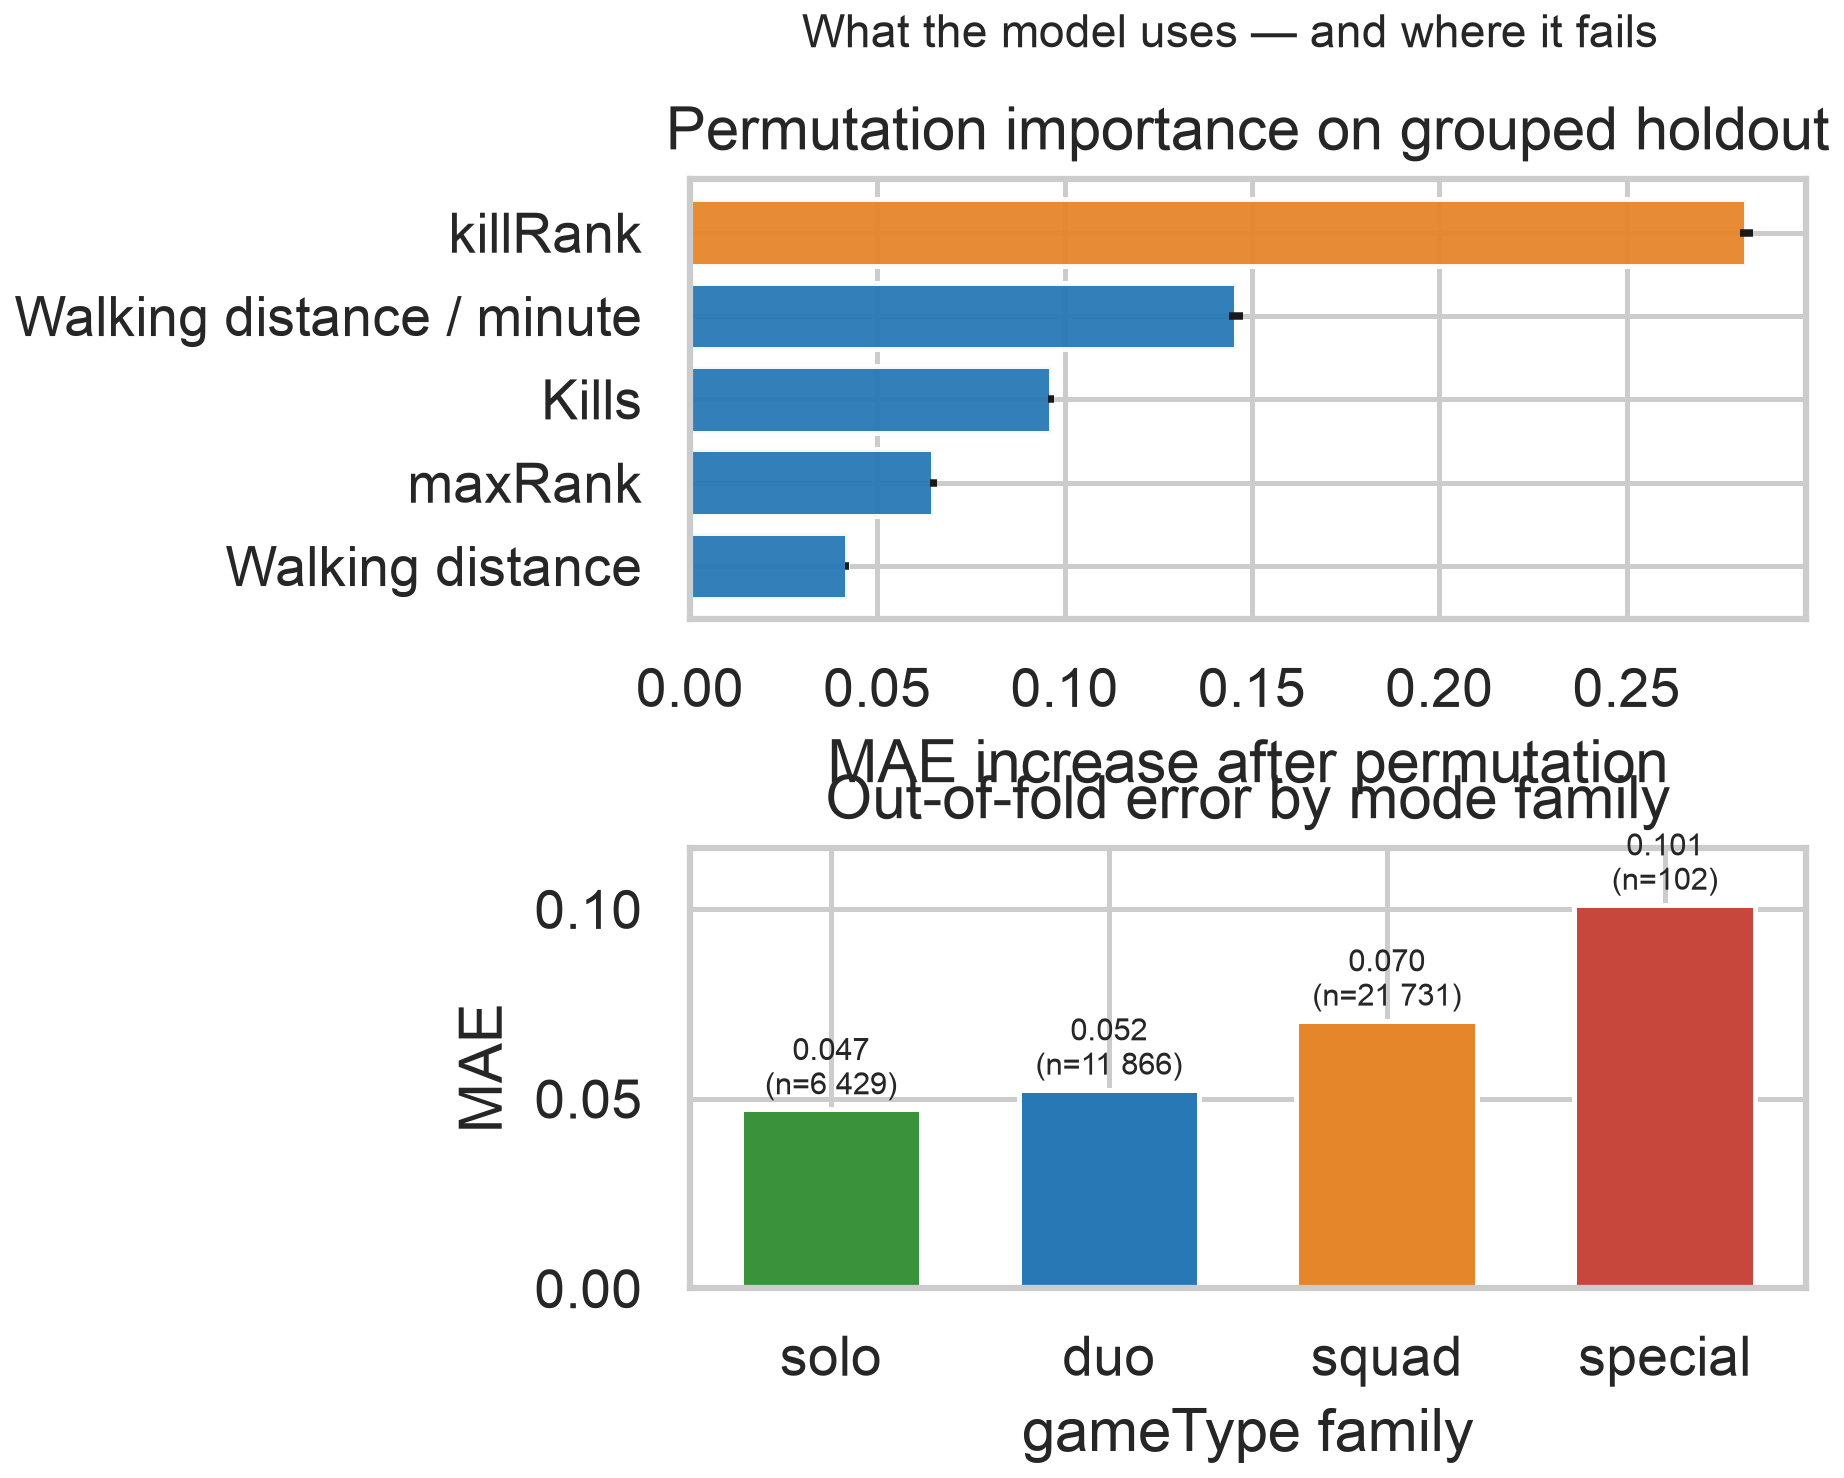
\includegraphics[width=0.88\columnwidth]{04_interpretation_errors.png}
\caption{What the model uses and where it fails. Importance confirms the role
of kill ranking and mobility; error grows in less represented, more complex
modes.}
\label{fig:interpretation}
\end{figure}

\textbf{Extreme errors complement mean MAE.} Out-of-fold predictions are
generally centered around the target, but residuals reveal regression to the
mean. On target band $[0.9,1]$, MAE rises to 0.0811 and bias reaches $-0.0755$:
the best rankings are underestimated on average. Two solo cases reach absolute
error 1.0 despite \code{maxRank=18}, zero kills, zero distance, and seven
weapons. Missing match context, atypical rows, or label noise may explain this
contrast; I retain those cases because deleting them after observing error would
bias evaluation.

\begin{figure}[!t]
\centering
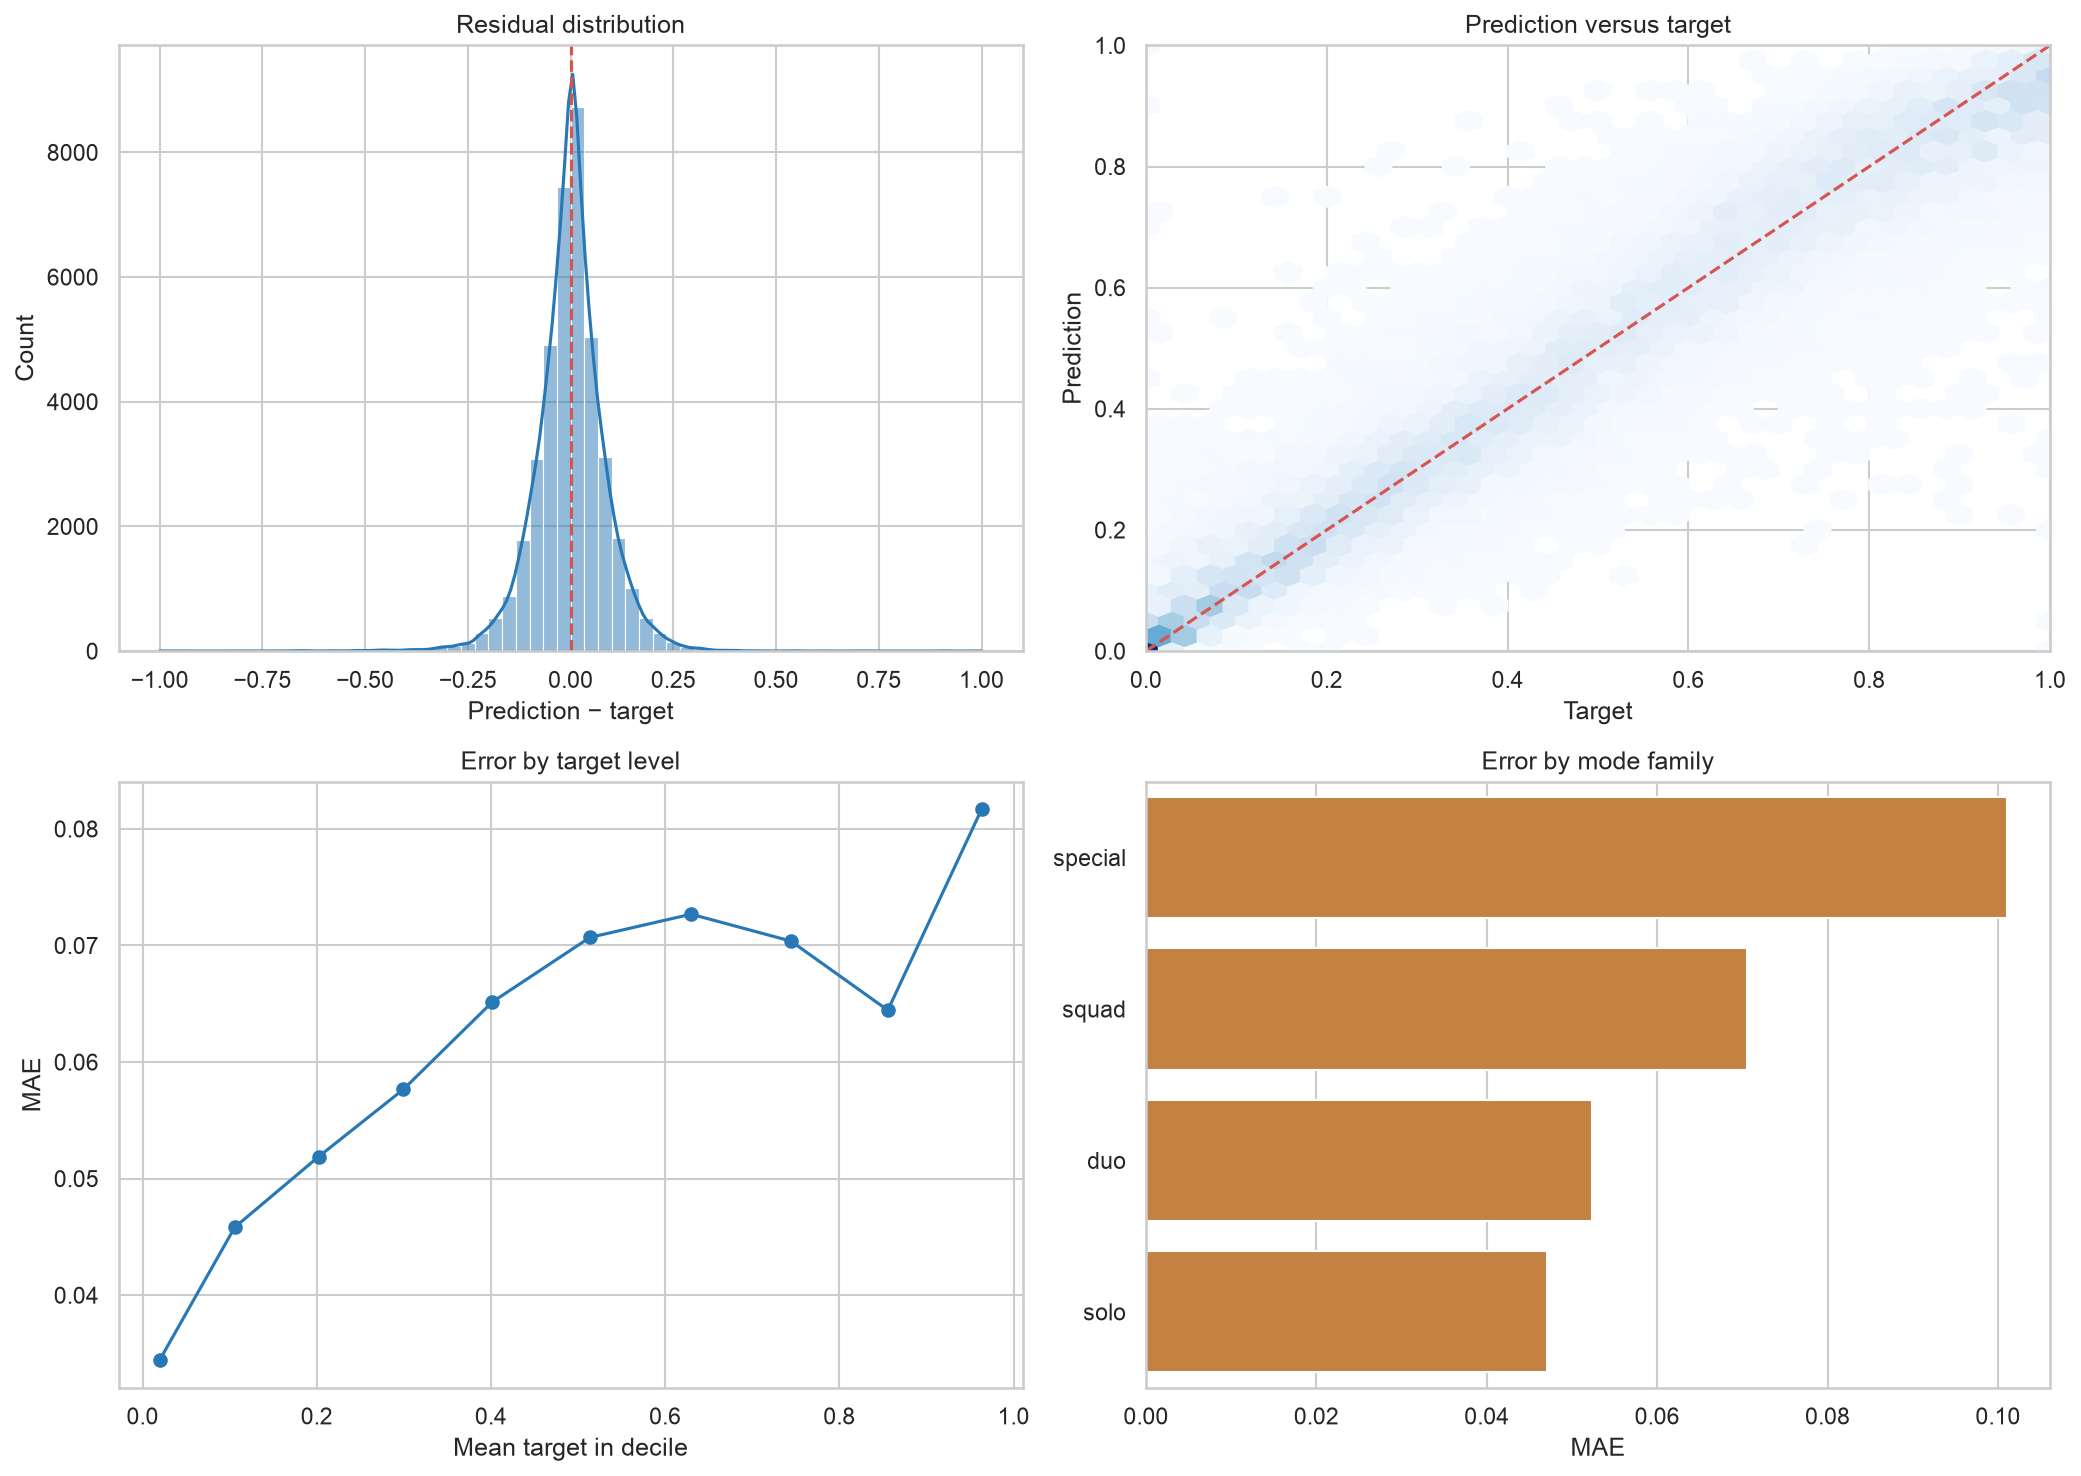
\includegraphics[width=0.96\columnwidth]{11_error_diagnostics.png}
\caption{Grouped-holdout residual analysis. Most errors remain near zero, but
performance degrades at the highest targets and in under-represented modes.}
\label{fig:error-outliers}
\end{figure}

\textbf{This result remains strictly post-match.} All available statistics are
post-match, inconsistent dates prevent credible future validation, rosters and
matches are incomplete, and test has no target, so performance drift is
unknown. A production version would require decision-time snapshots, complete
teams, a coherent match date, and a genuinely labeled future batch.

\noindent\textbf{Conclusion.} I connect problem understanding, quality checks,
outliers, exploration, validation, modeling, and interpretation. CatBoost
achieves 0.06080 MAE with an explicit, reproducible grouped protocol, while the
remaining extreme errors underline incomplete collective and temporal context.

\end{document}
